\documentclass[aspectratio=169,10pt]{beamer}

% ==========================================
% PAQUETES
% ==========================================
\usepackage[utf8]{inputenc}
\usepackage[T1]{fontenc}
\usepackage[spanish]{babel}
\usepackage{amsmath,amssymb}
\usepackage{graphicx}
\usepackage{booktabs}
\usepackage{array}
\usepackage{tikz}
\usepackage{hyperref}

\usetikzlibrary{arrows.meta,positioning}
\graphicspath{{figuras/}}

% ==========================================
% IDENTIDAD VISUAL ICESI
% ==========================================

\definecolor{AzulIcesi}{HTML}{5454E9}
\definecolor{VerdeIcesi}{HTML}{4CB979}
\definecolor{AmarilloIcesi}{HTML}{E4EB60}
\definecolor{MoradoIcesi}{HTML}{865CF0}

\definecolor{GrisFondo}{HTML}{F4F5F7}
\definecolor{GrisTexto}{HTML}{596273}
\definecolor{GrisClaro}{HTML}{E5E7EB}

% ==========================================
% CONFIGURACIÓN BEAMER
% ==========================================

\usetheme{default}

\setbeamertemplate{navigation symbols}{}

\setbeamercolor{normal text}{
 fg=black,
 bg=white
}

\setbeamercolor{structure}{
 fg=AzulIcesi
}

\setbeamercolor{frametitle}{
 fg=AzulIcesi,
 bg=white
}

\setbeamercolor{block title}{
 fg=white,
 bg=AzulIcesi
}

\setbeamercolor{block body}{
 fg=black,
 bg=GrisFondo
}

\setbeamercolor{itemize item}{
 fg=VerdeIcesi
}

\setbeamercolor{enumerate item}{
 fg=AzulIcesi
}

\setbeamercolor{alerted text}{
 fg=AzulIcesi
}

\setbeamerfont{frametitle}{
 size=\large,
 series=\bfseries
}

\setbeamertemplate{itemize item}{
 \raise0.2ex\hbox{\small$\blacktriangleright$}
}

\setbeamertemplate{itemize subitem}{
 \scriptsize$\bullet$
}

% ==========================================
% TÍTULO DE DIAPOSITIVAS
% ==========================================

\setbeamertemplate{frametitle}{
 \vspace{0.25cm}
 \insertframetitle
 \par
 \vspace{0.12cm}
 {\color{AzulIcesi}\rule{\linewidth}{1pt}}
 \vspace{-0.15cm}
}

% ==========================================
% PIE DE PÁGINA
% ==========================================
\logo{
    
\includegraphics[height=0.8cm]{logo_icesi.png}
}

\setbeamertemplate{footline}{
 \leavevmode
 \hbox{
  \begin{beamercolorbox}[
   wd=.82\paperwidth,
   ht=2.8ex,
   dp=1.2ex,
   leftskip=1em
  ]{normal text}
   \color{GrisTexto}
   \scriptsize
   UNIVERSIDAD ICESI
   \quad | \quad
   SEMP: SENSOR ELECTROMAGNÉTICO DE PROXIMIDAD
  \end{beamercolorbox}


 }
}

% ==========================================
% INFORMACIÓN DEL PROYECTO
% ==========================================

\title[SEMP]{
 SEMP: SENSOR ELECTROMAGNÉTICO DE PROXIMIDAD
}

\subtitle{
 Diseño y simulación de un sensor inductivo que detecta, identifica y ubica piezas metálicas
}


\author{
 Luis Ernesto Rodríguez\\
 Sebastián Santander Soto\\
 Kevin Lozano Gómez\\
 Juan Pablo Corchuelo\\
 Mateo López
}

\institute{
 Electromagnetismo\\
 Universidad Icesi
}

\date{
 Cali, Colombia\\
 2026
}

% ==========================================
% INICIO DEL DOCUMENTO
% ==========================================

\begin{document}

% ==========================================
% 1. PORTADA INSTITUCIONAL
% ==========================================

\begin{frame}[plain]

\vspace{0.2cm}

\IfFileExists{logo_icesi.png}{
 
\includegraphics[width=3.4cm]{logo_icesi.png}
}{
 {\color{AzulIcesi}
 \Large\bfseries Universidad Icesi}
}

\vspace{0.35cm}

{\color{VerdeIcesi}\rule{1.2cm}{2.5pt}}

\vspace{0.3cm}

{\color{AzulIcesi}
\fontsize{25}{30}\selectfont
\bfseries
SEMP: Sensor electromagnético de proximidad
}

\vspace{0.3cm}

{\color{GrisTexto}
\large
Diseño y simulación de un sensor inductivo que detecta, identifica y ubica piezas metálicas
}

\vspace{0.4cm}

{\color{AzulIcesi}\rule{\linewidth}{0.8pt}}

\vspace{0.3cm}

\textbf{Autores}

\vspace{0.1cm}

\begin{columns}[T]
\column{0.3\textwidth}
Luis Ernesto Rodríguez\\
Sebastián Santander Soto\\
Kevin Lozano Gómez
\column{0.3\textwidth}
Juan Pablo Corchuelo\\
Mateo López
\column{0.34\textwidth}
\small
Electromagnetismo\\
Universidad Icesi\\
{\color{GrisTexto}Cali, Colombia -- 2026}
\end{columns}

\vfill

\end{frame}

% ==========================================
% 2. CONTENIDO
% ==========================================

\begin{frame}{Contenido}

\begin{enumerate}
 \item Introducción
 \item Modelo teórico: esquema D.E.P.A.
 \item Implementación numérica
 \item Simulación computacional
 \item Resultados y discusión
 \item Conclusiones
 \item Referencias
\end{enumerate}

\end{frame}

% ==========================================
% 3. INTRODUCCIÓN
% ==========================================

\section{Introducción}

\begin{frame}{Introducción}

\begin{block}{Contexto del proyecto}
En las líneas de producción hay que detectar piezas metálicas sin tocarlas. Los sensores inductivos lo hacen con
un campo magnético variable y no les afectan el polvo, el aceite ni la suciedad.
\end{block}

\begin{itemize}
 \item \textbf{Problema:} una banda de autopartes lleva piezas de distintos metales mezcladas. No basta con
       saber que pasa una pieza: hay que saber \alert{de qué metal es} y \alert{a qué distancia está}.
 \item \textbf{Motivación:} clasificar y controlar la calidad con un solo sensor, sin contacto.
 \item \textbf{Propósito:} modelar el sensor desde Maxwell y construir un simulador interactivo.
 \item \textbf{Objetivos:}
 \begin{itemize}
  \item Deducir el modelo del sensor (Faraday, Ampère, circuito RL) y resolverlo analíticamente.
  \item Programar Euler y RK4 a mano y validar su convergencia.
  \item Simular la detección, la identificación del material y la estimación de la distancia.
 \end{itemize}
\end{itemize}

\end{frame}

% ==========================================
% 4. MODELO TEÓRICO
% ==========================================

\section{Modelo teórico}

\begin{frame}{Descripción del proceso: esquema D.E.P.A.}

Como en el espectrómetro de masas, el proceso se divide en etapas y cada una usa solo la matemática que necesita.

\vspace{0.25cm}

\begin{center}
\begin{tikzpicture}[node distance=0.35cm, >=Stealth]
 \node[align=center, text width=1.45cm] (ins) {\small\textbf{Insumos}\\[1pt]\scriptsize contexto de inicio};
 \node[right=0.35cm of ins, draw=AzulIcesi, fill=GrisFondo, rounded corners=2pt, minimum width=1.95cm,
       minimum height=1.45cm, align=center, text width=1.85cm] (D)
       {{\color{AzulIcesi}\bfseries\Large D}\\[2pt]{\scriptsize Detección\\material y distancia}};
 \node[right=0.35cm of D, draw=AzulIcesi, fill=GrisFondo, rounded corners=2pt, minimum width=1.95cm,
       minimum height=1.45cm, align=center, text width=1.85cm] (E)
       {{\color{AzulIcesi}\bfseries\Large E}\\[2pt]{\scriptsize Emisiones\\respuesta de la pieza}};
 \node[right=0.35cm of E, draw=AzulIcesi, fill=GrisFondo, rounded corners=2pt, minimum width=1.95cm,
       minimum height=1.45cm, align=center, text width=1.85cm] (P)
       {{\color{AzulIcesi}\bfseries\Large P}\\[2pt]{\scriptsize Propiedades\\$f$, energía, potencia}};
 \node[right=0.35cm of P, draw=AzulIcesi, fill=GrisFondo, rounded corners=2pt, minimum width=1.95cm,
       minimum height=1.45cm, align=center, text width=1.85cm] (A)
       {{\color{AzulIcesi}\bfseries\Large A}\\[2pt]{\scriptsize Alerta\\material, distancia}};
 \node[right=0.35cm of A, align=center, text width=1.45cm] (S)
       {\small\textbf{Solución}\\[1pt]\scriptsize contexto de impacto};
 \draw[->, thick, GrisTexto] (ins) -- (D);
 \draw[->, thick, AzulIcesi] (D) -- (E);
 \draw[->, thick, AzulIcesi] (E) -- (P);
 \draw[->, thick, AzulIcesi] (P) -- (A);
 \draw[->, thick, GrisTexto] (A) -- (S);
 \node[below=0.55cm of P, xshift=-1.3cm, draw=VerdeIcesi, thick, rounded corners=2pt, align=center,
       text width=5.2cm] (caso)
       {\scriptsize\textbf{Caso específico de estudio} $\rightarrow$ \textbf{Simulador}};
 \draw[->, GrisTexto] (ins.south) |- (caso.west);
 \draw[->, GrisTexto] (S.south) |- (caso.east);
\end{tikzpicture}
\end{center}

\vspace{0.1cm}

\begin{itemize}
 \item \textbf{Sistema:} bobina alimentada con corriente alterna y pieza metálica cercana.
 \item \textbf{Fenómeno:} el campo variable induce corrientes de Foucault (Faraday) cuyo campo se opone
       (Lenz): cambian $L$ y $R$.
\end{itemize}

\end{frame}

\begin{frame}{Descripción del proceso: variables y supuestos}

\begin{columns}[T]

\column{0.5\textwidth}

\textbf{Variables y parámetros}

\footnotesize
\begin{tabular}{@{}lll@{}}
\toprule
Magnitud & Símbolo & Tipo \\
\midrule
Campo magnético & $\vec B$ & vectorial \\
Campo eléctrico inducido & $\vec E$ & vectorial \\
Corrientes de Foucault & $\vec J=\sigma\vec E$ & vectorial \\
Corriente de la bobina & $i(t)$ & escalar \\
Inductancia, resistencia & $L$, $R$ & escalar \\
Conductividad, permeabilidad & $\sigma$, $\mu_r$ & escalar \\
Frecuencia, distancia & $\omega$, $d$ & escalar \\
\bottomrule
\end{tabular}

\column{0.46\textwidth}

\textbf{Supuestos del modelo}

\small
\begin{itemize}
 \item Régimen cuasi-estático: $\lambda = c/f = 300$ km frente a una bobina de 3 cm.
 \item Materiales lineales: $\sigma$ y $\mu_r$ constantes.
 \item Pieza como semiespacio (más ancha que la bobina y más gruesa que $3\delta$).
 \item Bobina de capa delgada, sin núcleo.
 \item Para cada posición de la pieza, $L$ y $R$ constantes.
\end{itemize}

\end{columns}

\end{frame}

\begin{frame}{Representación del proceso: el campo de la bobina y la pieza}

\begin{columns}[c]

\column{0.6\textwidth}

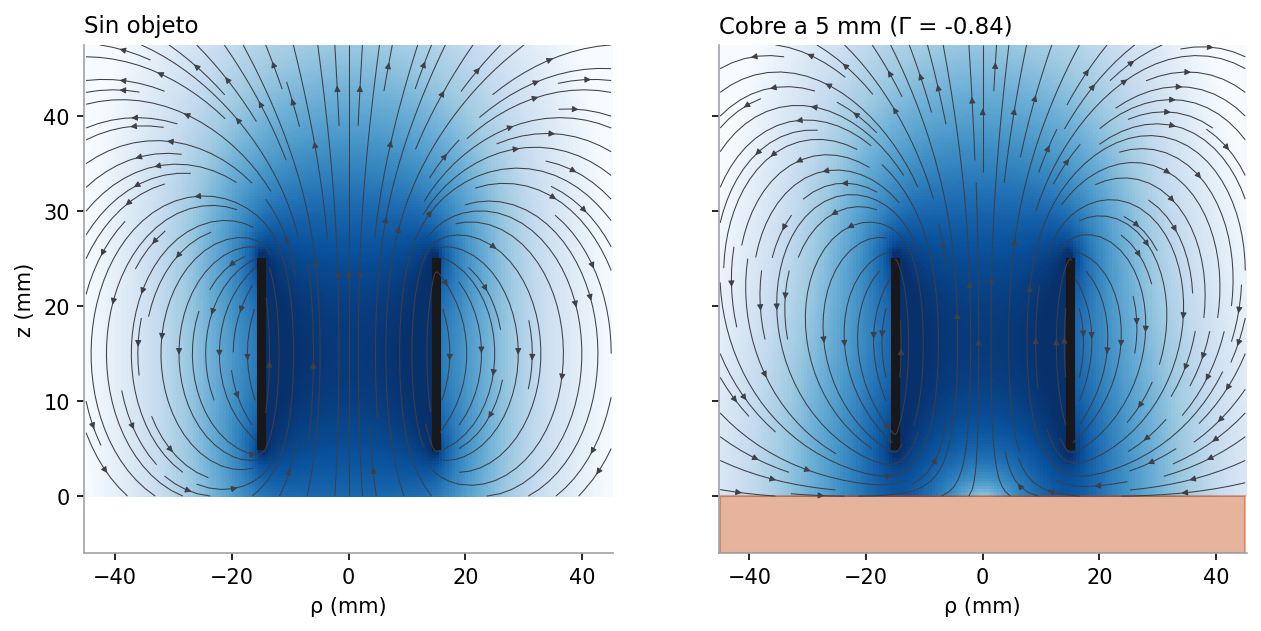
\includegraphics[width=\linewidth]{campo-magnetico.png}

\column{0.37\textwidth}

\small
\begin{enumerate}
 \item La bobina crea un campo $\vec B(t)$ que cambia mil veces por segundo.
 \item En la pieza aparece un campo $\vec E$ inducido (Faraday) y corrientes $\vec J=\sigma\vec E$.
 \item Esas corrientes crean un campo opuesto (Lenz): las líneas se \alert{acuestan} sobre el cobre.
 \item Parte del flujo deja de enlazar la bobina: $L$ baja. Las pérdidas por efecto Joule suben $R$.
\end{enumerate}

\end{columns}

\end{frame}

\begin{frame}{Formalismo matemático: solo las ecuaciones de Maxwell necesarias}

\begin{columns}[T]

\column{0.52\textwidth}

\textbf{Faraday} (la central): induce las corrientes en la pieza y la fem de la bobina
\[
 \oint_C \vec E\cdot d\vec l = -\frac{d\Phi_B}{dt},\qquad \Phi_B = \vec B\cdot\vec A
\]

\textbf{Ampère} sin corriente de desplazamiento ($\omega\varepsilon_0/\sigma\approx10^{-18}$)
\[
 \oint_C \vec B\cdot d\vec l = \mu_0 I_{enc}
\]

\textbf{Gauss magnética}, solo como condición de frontera
\[
 \oint_A \vec B\cdot d\vec A = 0 \;\Rightarrow\; B_z \text{ continuo en } z=0
\]

\column{0.44\textwidth}

En el metal queda una ecuación de difusión:
\[
 \nabla^2\vec A = j\omega\mu_0\mu_r\sigma\,\vec A
\]

con profundidad de penetración
\[
 \delta = \sqrt{\frac{2}{\omega\mu_0\mu_r\sigma}}
\]

\begin{block}{Condiciones de frontera}
\small
$B_z$ y $H_\rho$ continuos en la superficie; campos nulos lejos de la bobina.
Inicial: $i(0)=I_0$.
\end{block}

\end{columns}

\end{frame}

\begin{frame}{Formalismo matemático: el circuito RL, como el RC de clase}

\begin{columns}[T]

\column{0.5\textwidth}

Ley de mallas de Kirchhoff:
\[
 \varepsilon - iR - L\frac{di}{dt} = 0
\]

\textbf{Energizar} (escalón DC), por separación de variables:
\[
 \int_0^t\frac{dt}{\tau} = \int_0^{i}\frac{di}{i_{max}-i}
 \;\Rightarrow\;
 i(t)=i_{max}\left(1-e^{-t/\tau}\right)
\]
\[
 i_{max}=\frac{\varepsilon}{R},\qquad \tau=\frac{L}{R},\qquad i(\tau)=0.63\,i_{max}
\]

\column{0.46\textwidth}

\textbf{Alterna} $\varepsilon = V_0\sin\omega t$:
\[
 i(t) = \left[I_0 + I_p\sin\varphi\right]e^{-t/\tau} + I_p\sin(\omega t-\varphi)
\]
\[
 I_p = \frac{V_0}{\sqrt{R^2+\omega^2L^2}},\qquad \varphi=\arctan\frac{\omega L}{R}
\]

Inductancia de la bobina (Wheeler):
\[
 L_0 = \frac{\mu_0 N^2\pi a^2}{l+0.9a}
\]

\end{columns}

\vspace{0.15cm}

\begin{block}{Analogía}
\small
RC: $\tau=RC$, sube la carga $q$. \quad RL: $\tau=L/R$, sube la corriente $i$. Misma ecuación y misma curva.
\end{block}

\end{frame}

\begin{frame}{Formalismo matemático: efecto de la pieza y detección}

Solución de Dodd y Deeds para una bobina sobre un conductor:
\[
 \Delta Z = j\omega\pi\mu_0 a^2N^2\int_0^\infty J_1^2(\alpha a)\,\Gamma(\alpha)\,F^2(\alpha)\,d\alpha,
 \qquad
 \Gamma=\frac{\mu_r\alpha-\alpha_1}{\mu_r\alpha+\alpha_1},\quad \alpha_1=\sqrt{\alpha^2+j\omega\mu_0\mu_r\sigma}
\]
\[
 L_{\text{eff}} = L_0 + \frac{\operatorname{Im}\Delta Z}{\omega},\qquad R_{\text{eff}} = R_0 + \operatorname{Re}\Delta Z
\]

\begin{columns}[T]

\column{0.48\textwidth}

\begin{block}{D: detección}
\small
Hay pieza si $\dfrac{|I_p-I_{p,0}|}{I_{p,0}}\ \ge$ umbral (2 \%).
\end{block}

\column{0.48\textwidth}

\begin{block}{E y P: identificación}
\small
Con la \textbf{frecuencia}: la fase de $\Delta Z$ identifica el material.\\
Con la \textbf{potencia}: $|\Delta Z|$ da la distancia.
\end{block}

\end{columns}

\end{frame}

\begin{frame}{Caso de estudio: línea de autopartes}

\begin{columns}[T]

\column{0.55\textwidth}

\footnotesize
\begin{tabular}{@{}llrr@{}}
\toprule
Pieza & Material & $\sigma$ (S/m) & $\mu_r$ \\
\midrule
Tornillos & Acero al carbono & $6.0\times10^{6}$ & 100 \\
Cables & Cobre & $5.96\times10^{7}$ & 1 \\
Carcasas & Aluminio & $3.77\times10^{7}$ & 1 \\
Conectores & Latón & $1.5\times10^{7}$ & 1 \\
Abrazaderas & Inoxidable 304 & $1.45\times10^{6}$ & 1.02 \\
\bottomrule
\end{tabular}

\vspace{0.3cm}

\small
\textbf{Sensor de referencia:} $N=150$, $a=15$ mm, $l=20$ mm, $R_0=5\ \Omega$, $V_0=5$ V, $f=1$ kHz
(y 5 kHz); $L_0=0.60$ mH, $\tau_0=119\ \mu$s.

\column{0.41\textwidth}

\textbf{Requisitos}

\small
\begin{itemize}
 \item Avisar si una pieza pasa a menos de 8 mm.
 \item Identificar su material.
 \item Estimar su distancia.
 \item Avisar si no coincide con el catálogo (impureza).
\end{itemize}

\textbf{Alcance y limitaciones}

\begin{itemize}
 \item Movimiento lento frente al período.
 \item Sin núcleo de ferrita ni geometría finita.
\end{itemize}

\end{columns}

\end{frame}

% ==========================================
% 5. IMPLEMENTACIÓN NUMÉRICA
% ==========================================

\section{Implementación numérica}

\begin{frame}{Métodos de análisis numérico}

Problema de valor inicial $\;i' = f(t,i) = \dfrac{\varepsilon(t) - Ri}{L}$, $\;i(0)=I_0$, con paso $h=\Delta t$.

\begin{columns}[T]

\column{0.42\textwidth}

\textbf{Euler} (orden 1)
\[
 i_{k+1} = i_k + h\,f(t_k,i_k)
\]

\textbf{Estabilidad:} $|1-h/\tau|<1 \Rightarrow h<2\tau$

\vspace{0.2cm}

\textbf{Justificación:} la guía pide ambos; Euler es el punto de partida y RK4 el estándar de precisión.

\column{0.54\textwidth}

\textbf{Runge--Kutta 4} (orden 4)
\[
\begin{aligned}
 k_1 &= f(t_k,\, i_k) \\
 k_2 &= f\!\left(t_k+\tfrac h2,\, i_k+\tfrac h2k_1\right) \\
 k_3 &= f\!\left(t_k+\tfrac h2,\, i_k+\tfrac h2k_2\right) \\
 k_4 &= f(t_k+h,\, i_k+hk_3) \\
 i_{k+1} &= i_k + \tfrac h6\,(k_1+2k_2+2k_3+k_4)
\end{aligned}
\]

\end{columns}

\begin{block}{Criterios de precisión}
\small
$e_{abs}=\max_k|i_k-i(t_k)|$, \quad $e_{rel}=e_{abs}/\max|i|$, \quad
orden observado $p=\dfrac{\ln(e_k/e_{k+1})}{\ln(h_k/h_{k+1})}$
\end{block}

\end{frame}

\begin{frame}{Procedimiento computacional}

\begin{columns}[T]

\column{0.48\textwidth}

\begin{itemize}
 \item \textbf{Herramientas:} Python, NumPy, SciPy, SymPy, Matplotlib, Plotly y Streamlit.
 \item \textbf{Datos de entrada:} $N$, $a$, $l$, $R_0$, $V_0$, $f$, material, $d$, umbral, $I_0$.
 \item \textbf{Parámetros de cálculo:} pasos por ciclo (o por $\tau$) y duración.
 \item \textbf{Validación:}
 \begin{itemize}
  \item solución exacta y \texttt{solve\_ivp} de SciPy;
  \item 10 pruebas automáticas;
  \item balance de energía: error $5\times10^{-7}$;
  \item ejercicio RC de clase con el mismo código.
 \end{itemize}
\end{itemize}

\column{0.48\textwidth}

\begin{block}{Algoritmo}
\scriptsize
\textbf{1.} Leer parámetros de la bobina, la fuente y la pieza.\\
\textbf{2.} Calcular $L_0$ (Wheeler).\\
\textbf{3.} Calcular $\Delta Z$ (integral de Dodd--Deeds) y obtener $L_{\text{eff}}$, $R_{\text{eff}}$.\\
\textbf{4.} Integrar $i'=f(t,i)$ con Euler y RK4.\\
\textbf{5.} Comparar con la solución exacta: errores y orden.\\
\textbf{6.} Medir amplitud y fase $\rightarrow$ $\Delta Z$ medido.\\
\textbf{7.} Buscar la curva de material más cercana en el plano de impedancia $\rightarrow$ material y distancia.\\
\textbf{8.} Emitir la alerta con histéresis.
\end{block}

\end{columns}

\end{frame}

\begin{frame}{Convergencia de Euler y RK4}

\begin{columns}[T]

\column{0.6\textwidth}

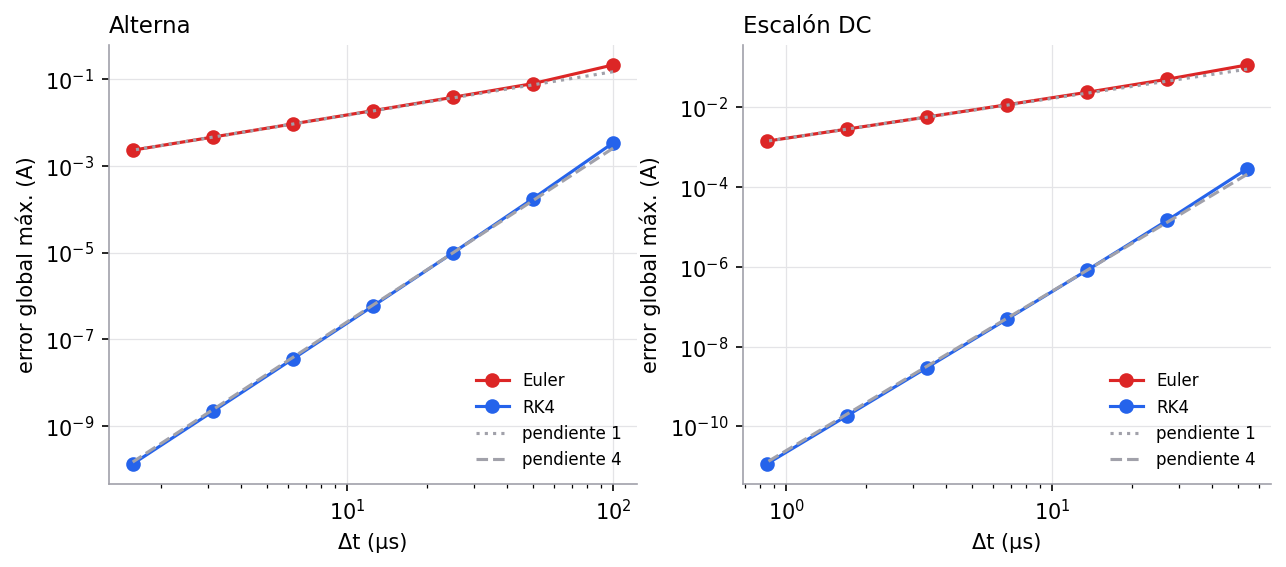
\includegraphics[width=\linewidth]{convergencia.png}

\column{0.37\textwidth}

\footnotesize
\begin{tabular}{@{}rrr@{}}
\toprule
Pasos/ciclo & Euler $e_{rel}$ & RK4 $e_{rel}$ \\
\midrule
10 & 25.6 \% & 0.41 \% \\
40 & 4.48 \% & $1.2\times10^{-3}$ \% \\
160 & 1.09 \% & $4.2\times10^{-6}$ \% \\
\bottomrule
\end{tabular}

\vspace{0.3cm}

\small
\begin{itemize}
 \item Orden medido: \textbf{1.01} (Euler) y \textbf{4.02} (RK4).
 \item Al dividir $h$ entre 2, el error de RK4 baja 16 veces.
 \item Para un 1 \% de error: Euler necesita 160 pasos por ciclo; RK4, 10.
\end{itemize}

\end{columns}

\end{frame}

% ==========================================
% 6. SIMULACIÓN COMPUTACIONAL
% ==========================================

\section{Simulación computacional}

\begin{frame}{Modelo de simulación}

\begin{columns}[T]

\column{0.48\textwidth}

\begin{itemize}
 \item \textbf{Estructura:} app web en Streamlit con 8 pestañas, de Modelo a Identificación.
 \item \textbf{Control:} espiras, radio, frecuencia, voltaje, material, distancia y umbral.
 \item \textbf{Escenarios:} 5 materiales; alterna o escalón DC; pieza fija o en movimiento.
 \item \textbf{Ejecución:} ruido de medida, promedios, una o dos frecuencias, paso $\Delta t$.
 \item \textbf{Herramientas:} Plotly y Matplotlib.
\end{itemize}

\column{0.48\textwidth}

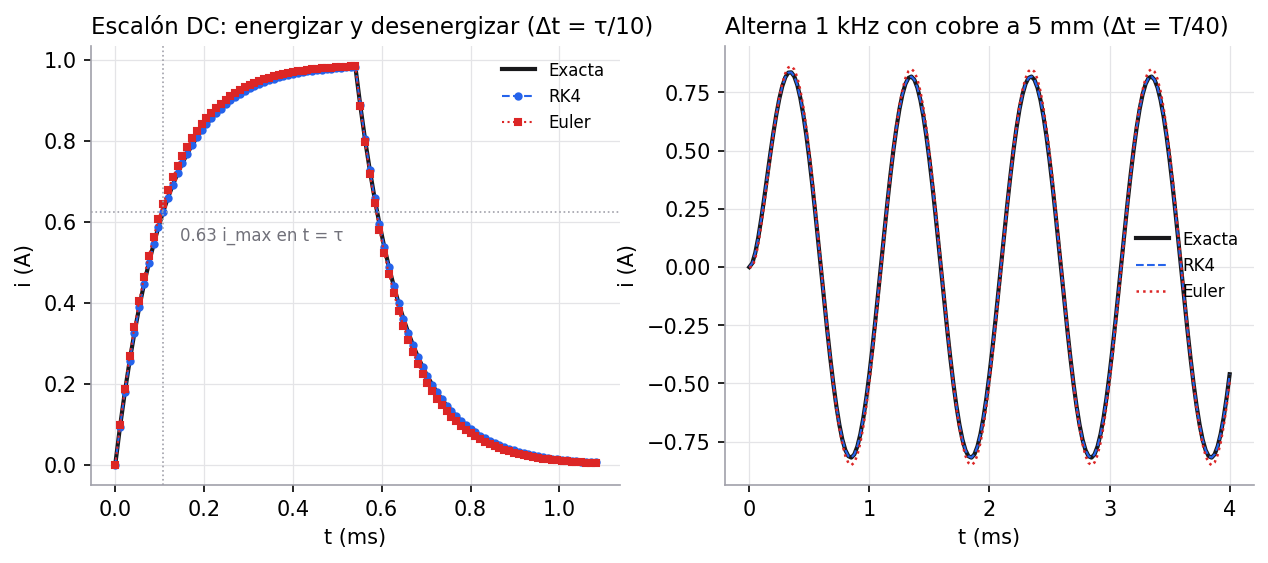
\includegraphics[width=\linewidth]{respuesta-temporal.png}

\scriptsize
\color{GrisTexto}
Izquierda: energizar y desenergizar la bobina ($\Delta t=\tau/10$). Derecha: alterna a 1 kHz con cobre a 5 mm.

\end{columns}

\end{frame}

\begin{frame}{Resultados de la simulación: parámetros y escenarios}

\begin{columns}[T]

\column{0.55\textwidth}

\begin{block}{Representación gráfica}
\centering
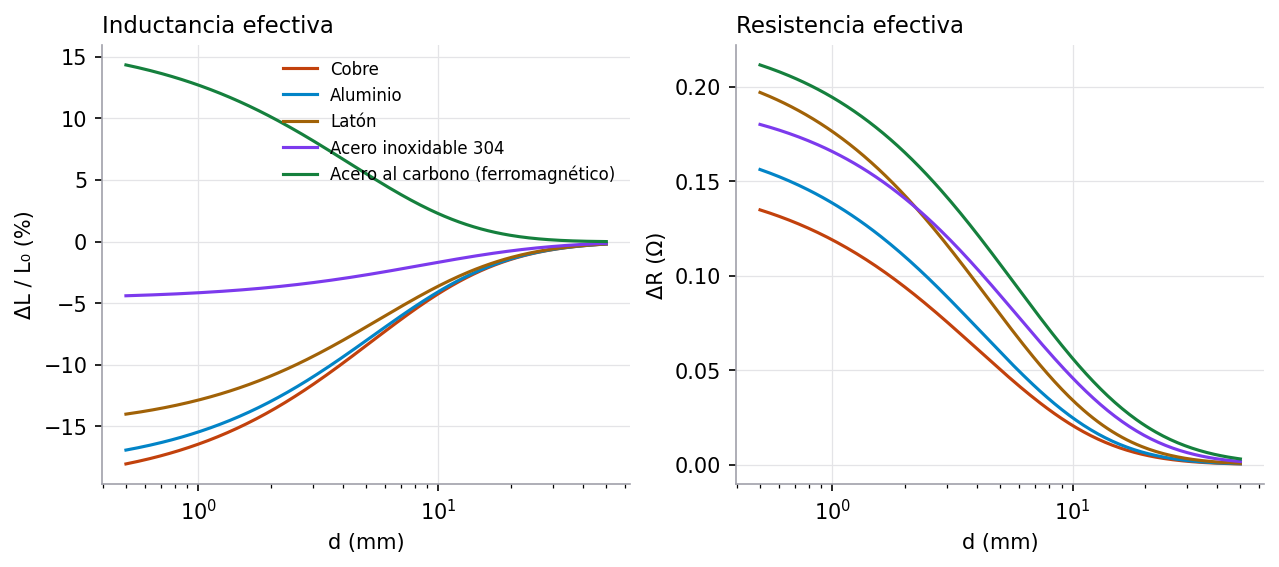
\includegraphics[height=2.75cm]{parametros-vs-distancia.png}

\vspace{0.05cm}

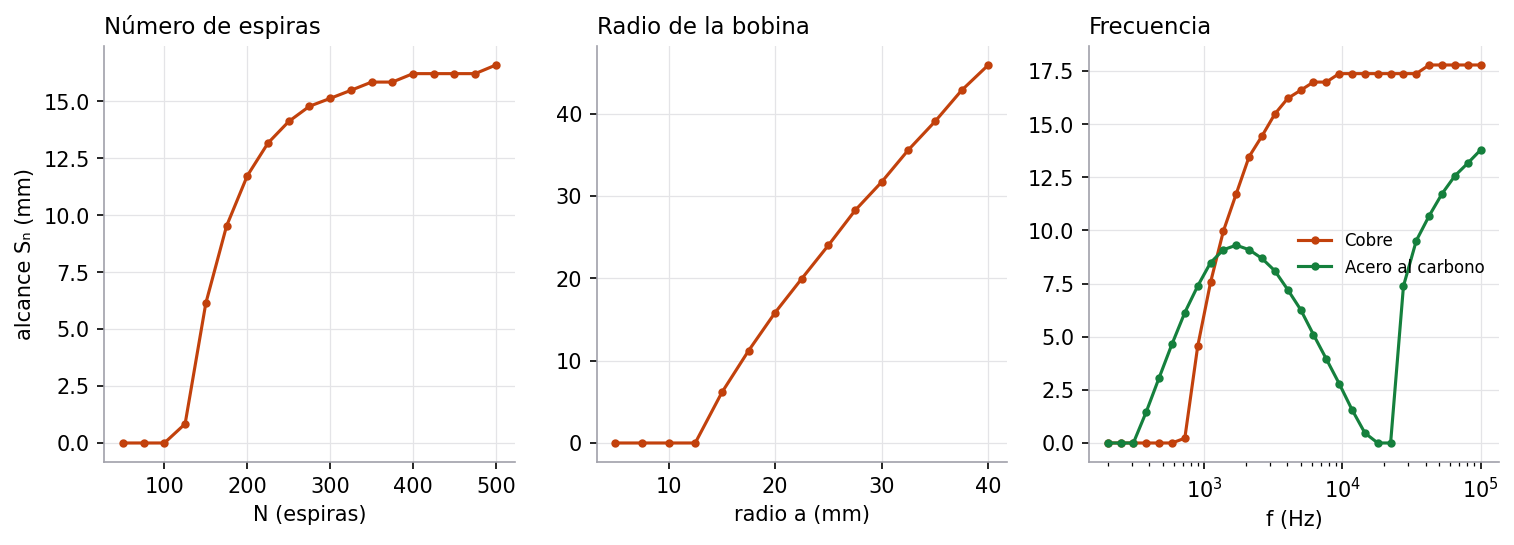
\includegraphics[height=2.2cm]{escenarios-alcance.png}
\end{block}

\column{0.42\textwidth}

\textbf{Observaciones}

\small
\begin{itemize}
 \item El cobre baja $L$ un 8.5 \% a 5 mm (apantallamiento); el acero la sube un 5.5 \% (magnetización).
 \item El efecto desaparece a una distancia del orden del radio: el campo cae como $1/z^3$ (dipolo).
 \item El alcance crece con el radio y con $N$.
 \item \alert{Frecuencia ciega} del acero cerca de 20 kHz: los dos efectos se cancelan.
\end{itemize}

\end{columns}

\end{frame}

\begin{frame}{Resultados de la simulación: identificación del material}

\begin{columns}[T]

\column{0.6\textwidth}

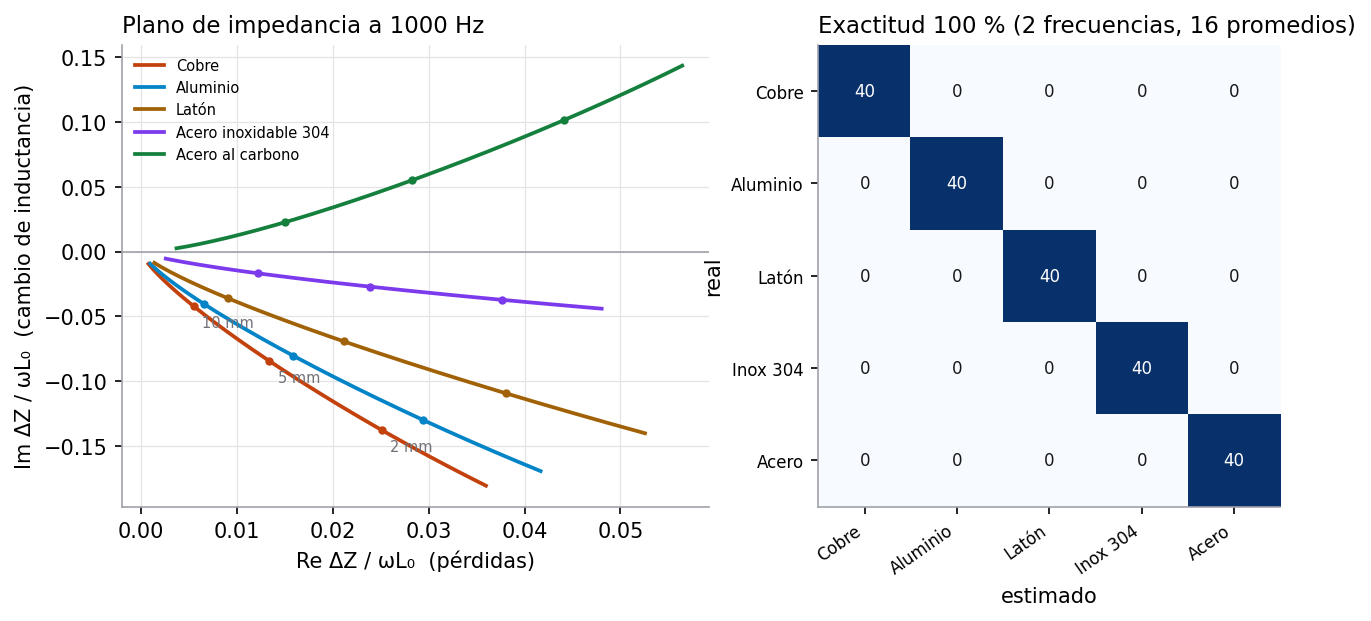
\includegraphics[width=\linewidth]{identificacion.png}

\column{0.37\textwidth}

\footnotesize
\begin{tabular}{@{}lrr@{}}
\toprule
Configuración & Material & Ferroso \\
\midrule
1 frecuencia & 84 \% & 100 \% \\
2 frecuencias & 89 \% & 100 \% \\
1 frec., 16 promedios & 100 \% & 100 \% \\
2 frec., 16 promedios & 100 \% & 100 \% \\
\bottomrule
\end{tabular}

\vspace{0.25cm}

\small
\begin{itemize}
 \item La fase separa ferrosos (positiva) de no ferrosos (negativa).
 \item Cobre, aluminio y latón exigen poco ruido.
 \item Error de distancia: 0.03 mm.
\end{itemize}

\end{columns}

\end{frame}

% ==========================================
% 7. RESULTADOS Y DISCUSIÓN
% ==========================================

\section{Resultados y discusión}

\begin{frame}{Resultados principales}

\begin{columns}[T]

\column{0.5\textwidth}

\begin{itemize}
 \item \textbf{Modelo teórico:} $L_0=0.60$ mH (la fórmula ideal da 67 \% de más); $\delta_{Cu}=2.1$ mm a 1 kHz.
 \item \textbf{Análisis numérico:} órdenes 1.01 y 4.02; balance de energía con error $5\times10^{-7}$.
 \item \textbf{Simulación:} alcance de 6.1 mm con cobre; identificación del 100 \% con dos frecuencias.
 \item \textbf{Comparación:} RK4 coincide con la solución exacta y con SciPy; el ejercicio RC de clase da
       $\tau=12$ s y $q_{max}=1.8$ mC.
\end{itemize}

\column{0.46\textwidth}

\begin{block}{Resultados (d = 5 mm, f = 1 kHz)}
\footnotesize
\begin{tabular}{@{}lrrr@{}}
\toprule
Material & $\Delta L/L_0$ & Fase $\Delta Z$ & $S_n$ \\
\midrule
Cobre & $-8.5$ \% & $-81^\circ$ & 6.1 mm \\
Aluminio & $-8.1$ \% & $-79^\circ$ & 5.2 mm \\
Latón & $-6.9$ \% & $-73^\circ$ & 1.5 mm \\
Inox 304 & $-2.7$ \% & $-49^\circ$ & -- \\
Acero & $+5.5$ \% & $+63^\circ$ & 7.9 mm \\
\bottomrule
\end{tabular}
\end{block}

\end{columns}

\end{frame}

\begin{frame}{Discusión}

\begin{itemize}
 \item \textbf{Teoría y simulación:} los casos límite se cumplen (conductor perfecto $\Gamma\to-1$, ferromagnético
       $L$ aumenta, pieza lejana sin efecto) y las curvas numéricas coinciden con las exactas.
 \item \textbf{Evaluación del modelo:} ordenando los metales por pérdidas ($\Delta R$) se obtiene el mismo orden de
       detección que publican los fabricantes; por eso los sensores reales miden pérdidas con un oscilador LC.
 \item \textbf{Impacto:} un solo sensor separa tornillos de acero, cables de cobre y conectores de latón;
       respuesta de 3.5 ms, unas 8\,500 piezas por minuto.
 \item \textbf{Limitaciones:}
 \begin{itemize}
  \item pieza infinita y bobina sin núcleo (un modelo de elementos finitos resolvería la geometría real);
  \item un cobre con el 60 \% de su conductividad es indistinguible del aluminio;
  \item promediar mejora la exactitud pero alarga la medición (96 ms con 16 promedios).
 \end{itemize}
\end{itemize}

\end{frame}

% ==========================================
% 8. CONCLUSIONES
% ==========================================

\section{Conclusiones}

\begin{frame}{Conclusiones}

\begin{enumerate}
 \item \textbf{Hallazgos:} la fase del cambio de impedancia identifica el material y su magnitud da la distancia;
       el acero tiene una frecuencia ciega cerca de 20 kHz.
 \item \textbf{Objetivos:} el modelo se dedujo desde Faraday y Ampère, Euler y RK4 convergen con sus órdenes
       teóricos y el simulador detecta, identifica y ubica las piezas.
 \item \textbf{Aportes:} el circuito del sensor se resuelve igual que el RC de clase, y el mismo código resuelve
       ambos.
 \item \textbf{Limitaciones y mejoras:} medir pérdidas ($\Delta R$) en lugar de amplitud, usar dos frecuencias y una
       medición diferencial para detectar impurezas.
 \item \textbf{Trabajo futuro:} geometría finita de la pieza, núcleo de ferrita y validación con un prototipo real.
\end{enumerate}

\end{frame}

% ==========================================
% 9. REFERENCIAS
% ==========================================

\section{Referencias}

\begin{frame}{Referencias}

\footnotesize

\begin{thebibliography}{10}

\bibitem{dodd}
Dodd, C. V. y Deeds, W. E.
Analytical solutions to eddy-current probe-coil problems.
\textit{Journal of Applied Physics}, 39, 2829, 1968.

\bibitem{wheeler}
Wheeler, H. A.
Simple inductance formulas for radio coils.
\textit{Proceedings of the IRE}, 16, 1398, 1928.

\bibitem{griffiths}
Griffiths, D. J.
\textit{Introduction to Electrodynamics}, 4.\textsuperscript{a} ed.
Cambridge University Press, 2017.

\bibitem{clase}
Universidad Icesi, curso de Electromagnetismo.
Apuntes de clase: circuito RC, ley de Gauss, campos eléctricos en la materia y pantallas táctiles
capacitivas, 2026.

\bibitem{guia}
Universidad Icesi.
Guía de proyectos de Electromagnetismo, 2026.

\bibitem{iag}
Anthropic.
\textit{Claude} (modelo de lenguaje), usado como asistente de programación y redacción, 2026.

\end{thebibliography}

\end{frame}

% ==========================================
% 10. MATERIAL COMPLEMENTARIO
% ==========================================

\begin{frame}{Material complementario}

Los desarrollos numéricos y computacionales pueden consultarse en:

\begin{itemize}
 \item Código fuente: modelo físico, Euler y RK4, identificación y simulador.
 \item Pruebas automáticas y script que genera las figuras.
 \item Informe completo organizado por los criterios de la rúbrica.
 \item Simulador interactivo: \texttt{streamlit run app.py}.
\end{itemize}

\vspace{0.3cm}

\textbf{Repositorio del proyecto:}

\url{https://github.com/luisrodriguez-rgb/Proyecto-Final-Fisica}

\end{frame}

% ==========================================
% 11. CIERRE
% ==========================================

\begin{frame}[plain]

\vfill

\begin{center}

{\color{AzulIcesi}
\fontsize{30}{36}\selectfont
\bfseries
GRACIAS
}

\vspace{0.4cm}

{\color{VerdeIcesi}
\rule{1.5cm}{2pt}
}

\vspace{0.5cm}

{\large Preguntas y discusión}

\vspace{0.8cm}

\IfFileExists{logo_icesi.png}{
 
\includegraphics[width=2.8cm]{logo_icesi.png}
}{
 {\color{AzulIcesi}\bfseries Universidad Icesi}
}

\end{center}

\vfill

\end{frame}

\end{document}
